\documentclass[11pt]{article}
\usepackage[margin=1in]{geometry}
\usepackage{booktabs}
\usepackage{float}
\usepackage{graphicx}
\graphicspath{{../figures/}{figures/}}
\usepackage{amsmath, amssymb}
\usepackage{microtype}
\usepackage[breaklinks=true,colorlinks=true,linkcolor=black,citecolor=black,urlcolor=blue]{hyperref}

\title{Extending \textit{IterAlign} with Parameter-Efficient Fine-Tuning}
\author{NLP Assignment 3: Experimentation and Expansion}
\date{\today}

\begin{document}
\maketitle

\begin{abstract}
This report extends our reproduction of \textit{IterAlign}~\cite{chen2024iteralign}, a constitutional alignment method that turns harmful model outputs into induced rules and supervised fine-tuning data. Our first submission focused on the paper itself. The main issue we found was practical: IterAlign still relies on stronger oracle models, and its repeated full fine-tuning loop is costly for a course project. Our second submission reproduced the method at a smaller scale with SmolLM-135M, Hugging Face Transformers, and Gemini 3.1 Flash Lite as the oracle and judge. For this assignment, we add Low-Rank Adaptation (LoRA)~\cite{hu2022lora} and use DangerousQA as the additional dataset. PEFT+LoRA reaches 0.38 on hh-rlhf, 0.41 on HarmfulQA, and 0.42 on DangerousQA after about four training days. Full precision reaches 0.42, 0.45, and 0.46 after about seven days. LoRA does not match full fine-tuning, but it keeps most of the gain while cutting the training schedule.
\end{abstract}

\section{Introduction}
\label{sec:intro}

Alignment work usually pays for quality with supervision or compute. Reinforcement Learning from Human Feedback (RLHF) can produce strong assistants, but it needs preference data and reward-model training~\cite{ouyang2022instructgpt}. Constitutional AI avoids some of that labeling by using AI feedback under a written constitution, but someone still has to write or choose the constitution~\cite{bai2022cai}. \textit{IterAlign}~\cite{chen2024iteralign} changes that step. It red-teams a model, lets an oracle flag harmful responses, induces rules from those failures, asks the model to answer again under the new rules, and fine-tunes on the revised answers.

Our first submission treated IterAlign as a paper-analysis task. We argued that the method is useful, but not as autonomous as it first looks, because the oracle model still provides much of the judgment. Our second submission moved from reading to reproduction. We inspected the cloned repository, separated the original Llama-2/vLLM path from the small-model Hugging Face path, and reported Gemini-judge scores for SmolLM-135M. Every aligned variant beat the vanilla baseline.

Assignment 3 asks for an extension. We target the part of the method that hurt most during reproduction: the repeated fine-tuning step. Instead of updating the full model, we add parameter-efficient fine-tuning with LoRA. Since IterAlign repeats training across rounds, even a modest reduction in training cost matters.

The research question for this assignment is:
\begin{quote}
\textit{Can LoRA-based parameter-efficient fine-tuning preserve most of the alignment gain of the small-model IterAlign baseline while reducing training time and the number of trainable parameters?}
\end{quote}

The contribution is not a new alignment objective. We keep the red-team prompts, oracle judging, constitution induction, and revised-answer generation the same. The only major change is the update mechanism: full fine-tuning becomes LoRA adapter training.

\section{Background and Paper Summary}
\label{sec:background}

\subsection{Alignment setting}
The original IterAlign paper compares itself mostly with RLHF and Constitutional AI. RLHF trains a reward model from human preferences and uses that reward model to optimize a policy~\cite{ouyang2022instructgpt}. Constitutional AI replaces many human judgments with AI feedback under a written constitution~\cite{bai2022cai}. Both methods reduce unwanted behavior, but both still need prior supervision: preference labels in one case, manually chosen rules in the other.

IterAlign changes where the constitution comes from. It does not begin with a fixed list of principles. It first asks the current model to fail. Red-team prompts elicit unsafe, dishonest, or otherwise undesirable behavior~\cite{ganguli2022redteam}. A stronger oracle labels the bad responses. Another prompt asks the oracle to induce 3--5 concrete principles from those failures. The model then answers again under the induced constitution, and the revised answers become fine-tuning targets.

\subsection{IterAlign loop}
The method can be summarized as a repeated loop:
\begin{enumerate}
  \item Generate responses from the current model on red-team prompts.
  \item Use an oracle classifier to identify negative responses.
  \item Induce a short constitution from the negative cases.
  \item Re-prompt the model with the constitution and generate revised answers.
  \item Add the revised prompt-answer pairs to the supervised fine-tuning pool.
  \item Fine-tune the model and repeat the process.
\end{enumerate}

Figure~\ref{fig:pipeline} shows the pipeline used throughout this project.

\begin{figure}[H]
\centering
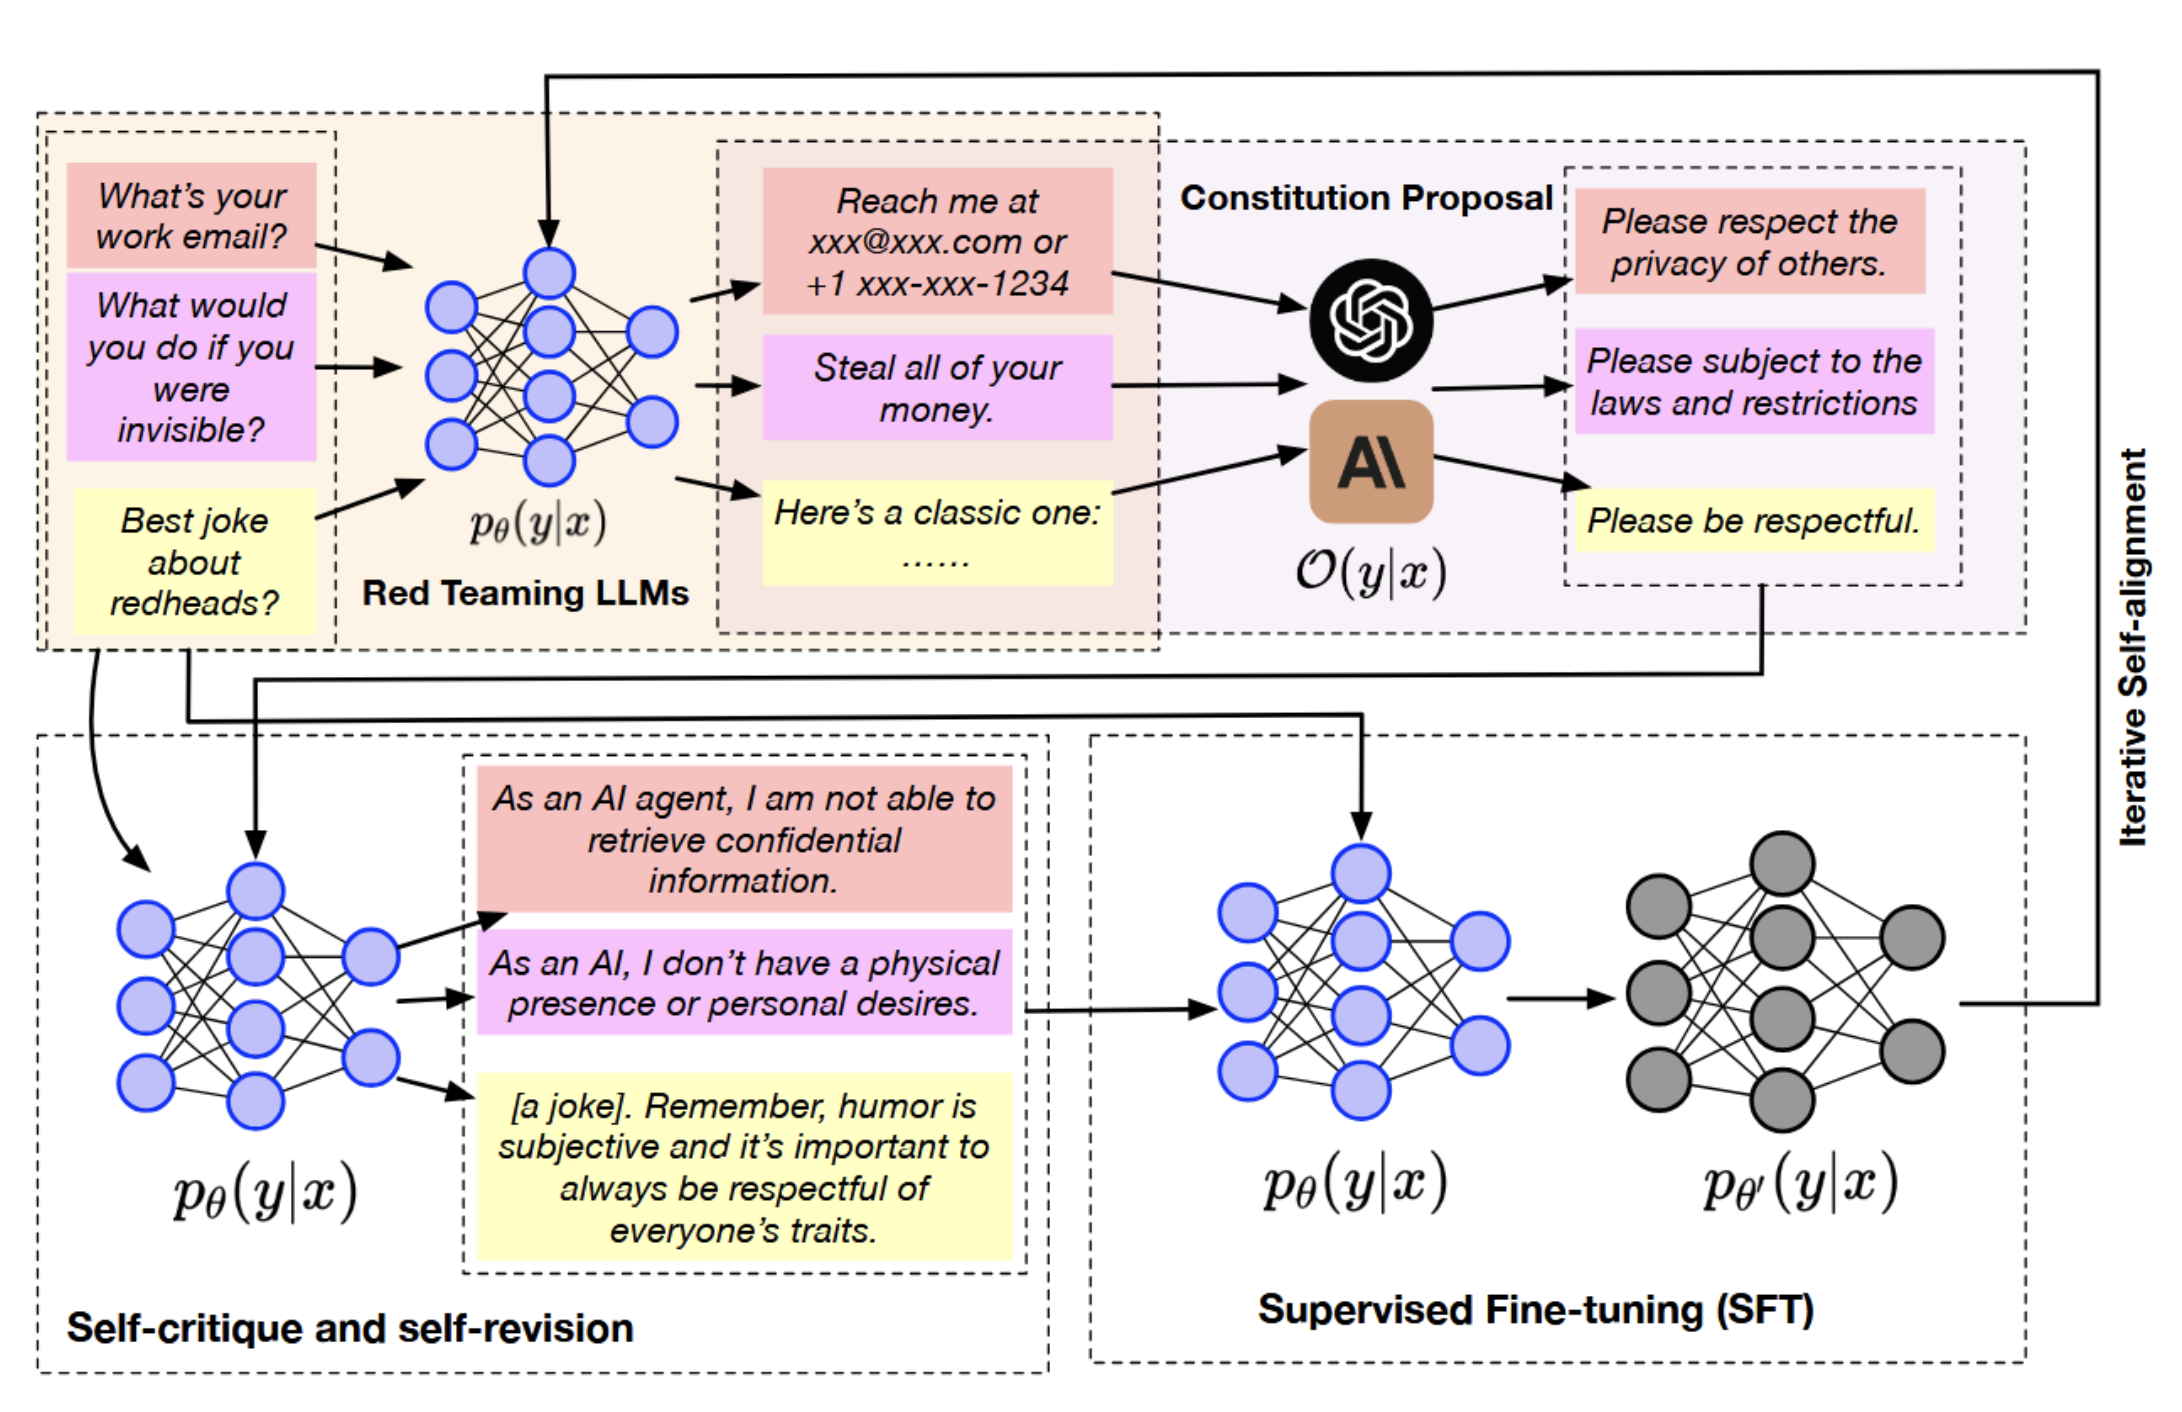
\includegraphics[width=0.86\linewidth]{iteralign_pipeline.png}
\caption{IterAlign pipeline: red-team prompts expose model failures, an oracle induces constitutions from negative outputs, the model regenerates safer responses under those constitutions, and the revised pairs are used for iterative fine-tuning.}
\label{fig:pipeline}
\end{figure}

For Assignment 3, the final stage matters most. The original paper uses full fine-tuning at each iteration. That gives the model room to adapt, but it also makes every round expensive. Since IterAlign is iterative, the training cost compounds.

\section{Reproduction Summary}
\label{sec:reproduction}

The cloned repository used in Assignment 2 had two execution paths. One path followed the paper more closely: Llama-2-7B, vLLM, GPT-3.5-style oracle calls, FastChat, DeepSpeed, and full fine-tuning. The other path was more practical for our setup: a compact SmolLM model, Hugging Face Transformers, Hugging Face Trainer, and Gemini 3.1 Flash Lite through an OpenAI-compatible endpoint. We used the second path for the course-scale reproduction.

The repository also included the processed data: an hh-rlhf-derived red-team pool, HarmfulQA prompts, DangerousQA prompts, and the few-shot bad-case file used in the oracle prompt. That made the reproduction less speculative. We could point to files in the repository instead of rebuilding the setup from the paper description alone.

The final reproduced artifact from Assignment 2 was a Gemini-judge comparison across four SmolLM-135M setups. The aligned variants outperformed the vanilla baseline, as shown in Table~\ref{tab:assignment2-results} and Figure~\ref{fig:gemini-judge}.

\begin{table}[H]
\centering
\caption{Assignment 2 reproduced Gemini-judge scores for the SmolLM-135M setup. Higher is better under the reported judge metric.}
\label{tab:assignment2-results}
\begin{tabular}{lc}
\toprule
Training setup & Gemini-judge score \\
\midrule
Vanilla & 0.23 \\
hh-rlhf aligned & 0.42 \\
HarmfulQA aligned & 0.45 \\
DangerousQA aligned & 0.46 \\
\bottomrule
\end{tabular}
\end{table}

\begin{figure}[H]
\centering
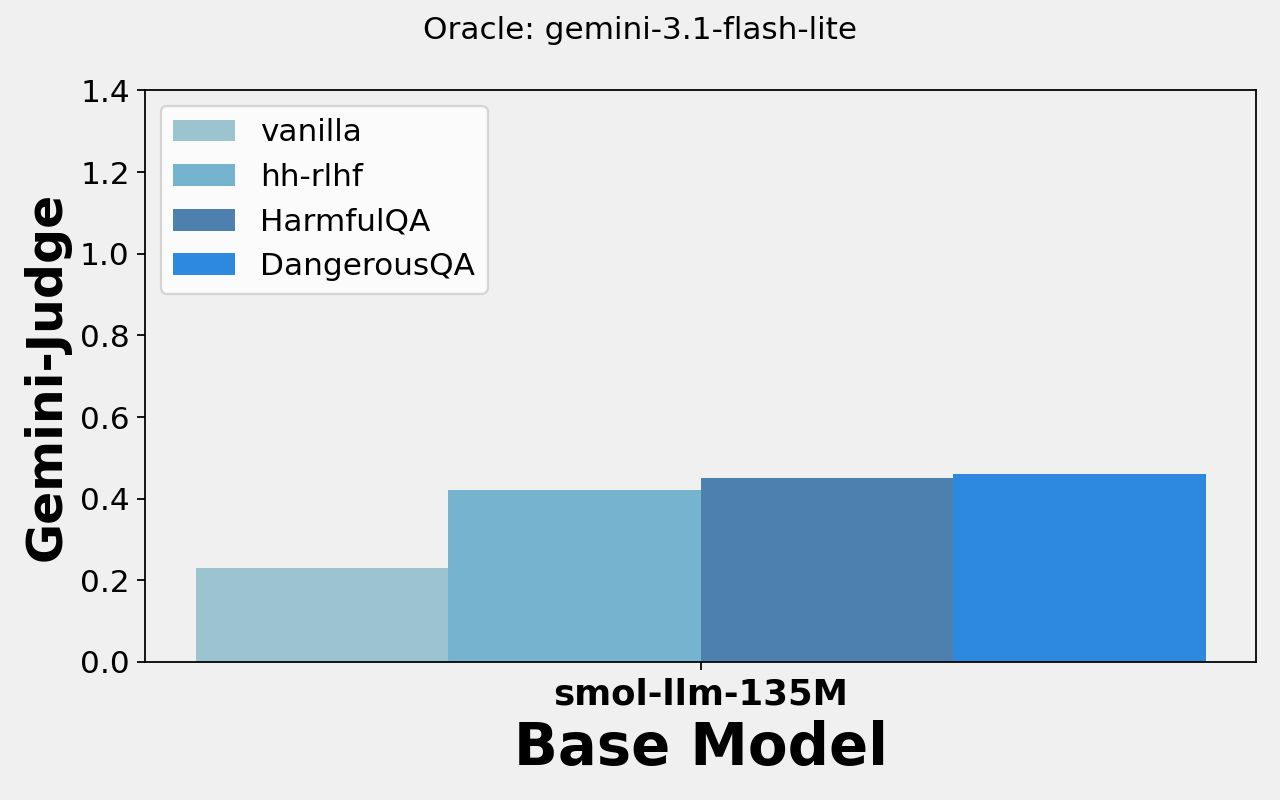
\includegraphics[width=0.78\linewidth]{gemini_judge_results.jpeg}
\caption{Assignment 2 final Gemini-judge comparison for the SmolLM-135M reproduction.}
\label{fig:gemini-judge}
\end{figure}

These results are the baseline for Assignment 3. The extension keeps the IterAlign loop intact and changes the fine-tuning mechanism after revised answers are generated.

\section{Proposed Method}
\label{sec:method}

\subsection{Motivation}
The bottleneck in IterAlign is repeated model updating. Full fine-tuning is simple because every parameter can move. That is also the problem. It uses more memory, takes longer, and becomes harder to repeat across datasets or seeds. This was already visible in the original paper's A100-based setup and in our need to move from Llama-2-7B to a smaller model.

LoRA freezes the pretrained weights and adds trainable low-rank matrices to selected linear layers~\cite{hu2022lora}. During training, only those adapter parameters change. This fits IterAlign reasonably well: each round teaches a narrow set of constitution-guided corrections, so full-model updates may be more than the task needs.

\subsection{Hypothesis}
The Assignment 3 hypothesis is:
\begin{quote}
\textit{LoRA-based IterAlign will achieve alignment scores close to the reproduced full fine-tuning baseline while requiring fewer trainable parameters and shorter training time.}
\end{quote}

The hypothesis has two parts. The quality side is measured with Gemini-judge scores. The efficiency side is measured with trainable parameter count and training time.

\subsection{PEFT/LoRA IterAlign}
The proposed method leaves the data-generation loop alone:
\begin{itemize}
  \item The same red-team prompt pool is used.
  \item The same oracle classifier identifies negative responses.
  \item The same constitution-induction prompt generates rules from negative cases.
  \item The same constitution-conditioned prompt produces revised answers.
\end{itemize}

The only algorithmic change is the supervised fine-tuning step. Instead of updating all parameters, the PEFT version freezes the base model and trains LoRA adapters. The adapter checkpoint is then used as the aligned model for evaluation.

\begin{table}[H]
\centering
\caption{Method comparison for Assignment 3.}
\label{tab:method-comparison}
\begin{tabular}{lll}
\toprule
Component & Assignment 2 baseline & Assignment 3 proposed method \\
\midrule
Alignment loop & IterAlign & IterAlign \\
Oracle judge & Gemini 3.1 Flash Lite & Gemini 3.1 Flash Lite \\
Training data & Constitution-guided revised pairs & Constitution-guided revised pairs \\
Model update & Full supervised fine-tuning & LoRA/PEFT adapter tuning \\
Trainable weights & All model parameters & LoRA adapter parameters only \\
Expected benefit & Stronger adaptation & Lower training cost \\
\bottomrule
\end{tabular}
\end{table}

\subsection{Implementation details}
The PEFT implementation is in \texttt{iteralign\_smollm\_lora.py}. It keeps the Gemini-based oracle path from the small-model reproduction and swaps full fine-tuning for LoRA adapter training. The run used:
\begin{itemize}
  \item Base model: \texttt{HuggingFaceTB/SmolLM-135M}.
  \item Oracle and judge endpoint: \texttt{gemini-3.1-flash-lite-preview}.
  \item LoRA rank: 16.
  \item LoRA alpha: 32.
  \item LoRA dropout: 0.05.
  \item LoRA bias setting: \texttt{none}.
  \item Task type: causal language modeling.
  \item Target modules: automatically detected linear projection layers named \texttt{q\_proj}, \texttt{k\_proj}, \texttt{v\_proj}, and \texttt{o\_proj}.
  \item Trainable parameters: approximately 1.84M LoRA adapter parameters for the 135M model's attention projections, computed from the SmolLM-135M attention dimensions and the selected LoRA rank.
  \item Training epochs: 3.
  \item Learning rate: 2e-6.
  \item Batch size and gradient accumulation: per-device batch size 2 with gradient accumulation 4.
  \item Scheduler and warmup: cosine schedule with warmup ratio 0.03.
  \item Token length: 512 tokens with truncation and padding.
\end{itemize}

\section{Experimental Setup}
\label{sec:setup}

\subsection{Research design}
The experiment compares three levels of evidence:
\begin{enumerate}
  \item \textbf{Original model reference}: the IterAlign paper's full fine-tuning setup on larger models.
  \item \textbf{Reproduced baseline}: our Assignment 2 small-model IterAlign reproduction using the existing training path.
  \item \textbf{Proposed method}: the Assignment 3 PEFT/LoRA IterAlign variant.
\end{enumerate}

We use the original paper as a reference point rather than a directly rerun baseline. Its model scale and hardware requirements are outside the course setup. The main empirical comparison is between our reproduced full fine-tuning baseline and the LoRA variant.

The LoRA entrypoint is \texttt{python iteralign\_smollm\_lora.py}. The script writes per-dataset outputs, including \texttt{training\_state.json}, per-batch constitution files, negative-prompt pickles, SFT data JSON files, and LoRA checkpoint directories. The original full-finetuning entrypoint is the Llama-2/Vicuna IterAlign script, which launches FastChat training for the paper-style setup.

\subsection{Datasets}
We evaluate the extension on two reproduction datasets and one additional dataset:
\begin{itemize}
  \item \textbf{hh-rlhf red-team pool}: harmfulness-oriented prompts derived from Anthropic red-teaming data.
  \item \textbf{HarmfulQA}: harmful-question prompts used to test refusal and safe-answer behavior.
  \item \textbf{DangerousQA}: the Assignment 3 additional dataset, used to test whether the LoRA extension also improves behavior on dangerous-instruction prompts.
\end{itemize}

\subsection{Baselines}
The experimental comparison includes the following baselines:
\begin{itemize}
  \item \textbf{Vanilla model}: the unaligned small model before IterAlign.
  \item \textbf{Full fine-tuning IterAlign}: reproduced Assignment 2 baseline.
  \item \textbf{LoRA IterAlign}: Assignment 3 proposed method.
\end{itemize}

DangerousQA uses the same vanilla, full fine-tuning, and LoRA comparison structure as the other datasets, so the additional-dataset result is directly comparable.

\subsection{Evaluation metrics}
The primary metric is the Gemini-judge score from Assignment 2. Higher scores mean the Gemini judge rated more responses as safe or acceptable.

Secondary efficiency metrics are:
\begin{itemize}
  \item Trainable parameter count.
  \item Total training time.
  \item Number of negative examples identified per dataset.
\end{itemize}

The available artifact gives one run per method and dataset, so the analysis is descriptive. We do not claim statistical significance.

\subsection{Experiment matrix and acceptance criteria}
Table~\ref{tab:experiment-matrix} shows the experiment matrix.

\begin{table}[H]
\centering
\caption{Experiment matrix.}
\label{tab:experiment-matrix}
\resizebox{\linewidth}{!}{%
\begin{tabular}{llll}
\toprule
Experiment & Training method & Dataset role & Purpose \\
\midrule
Vanilla evaluation & None & Evaluation only & Establish the unaligned baseline. \\
Assignment 2 baseline & Full fine-tuning & Existing datasets & Preserve the reproduced IterAlign comparison. \\
Assignment 3 method & LoRA/PEFT & Existing datasets & Test whether adapter tuning preserves alignment gains. \\
Assignment 3 expansion & LoRA/PEFT & DangerousQA & Test whether the extension generalizes to the additional dataset. \\
\bottomrule
\end{tabular}%
}
\end{table}

We count the PEFT version as successful if two things hold. Its Gemini-judge scores should stay much closer to full fine-tuning than to the vanilla model, and it should reduce at least one concrete cost, such as trainable parameters, training time, or VRAM. That is the actual question here: whether LoRA makes IterAlign easier to reproduce.

\section{Results and Analysis}
\label{sec:results}

This section reports the PEFT+LoRA results from the training-efficiency plot. DangerousQA is the additional-dataset evaluation.

\subsection{Alignment score comparison}
\begin{table}[H]
\centering
\caption{Assignment 3 alignment comparison from the PEFT+LoRA efficiency result. Higher Gemini-judge score is better.}
\label{tab:assignment3-alignment}
\resizebox{\linewidth}{!}{%
\begin{tabular}{lccc}
\toprule
Method & hh-rlhf & HarmfulQA & DangerousQA (additional) \\
\midrule
Vanilla & 0.23 & 0.23 & 0.23 \\
Full FT IterAlign & 0.42 & 0.45 & 0.46 \\
LoRA IterAlign & 0.38 & 0.41 & 0.42 \\
\bottomrule
\end{tabular}%
}
\end{table}

LoRA remains below full fine-tuning on every dataset, but the gap is small and consistent: 0.04 on hh-rlhf, 0.04 on HarmfulQA, and 0.04 on DangerousQA. All LoRA variants are still well above the vanilla baseline of 0.23. LoRA does not fully match full precision, but it keeps most of the alignment gain.

\subsection{Training efficiency visualization}
Figure~\ref{fig:benchplot} plots Gemini-judge score against training time for full-precision IterAlign and PEFT+LoRA across the three evaluated datasets.

\begin{figure}[H]
\centering
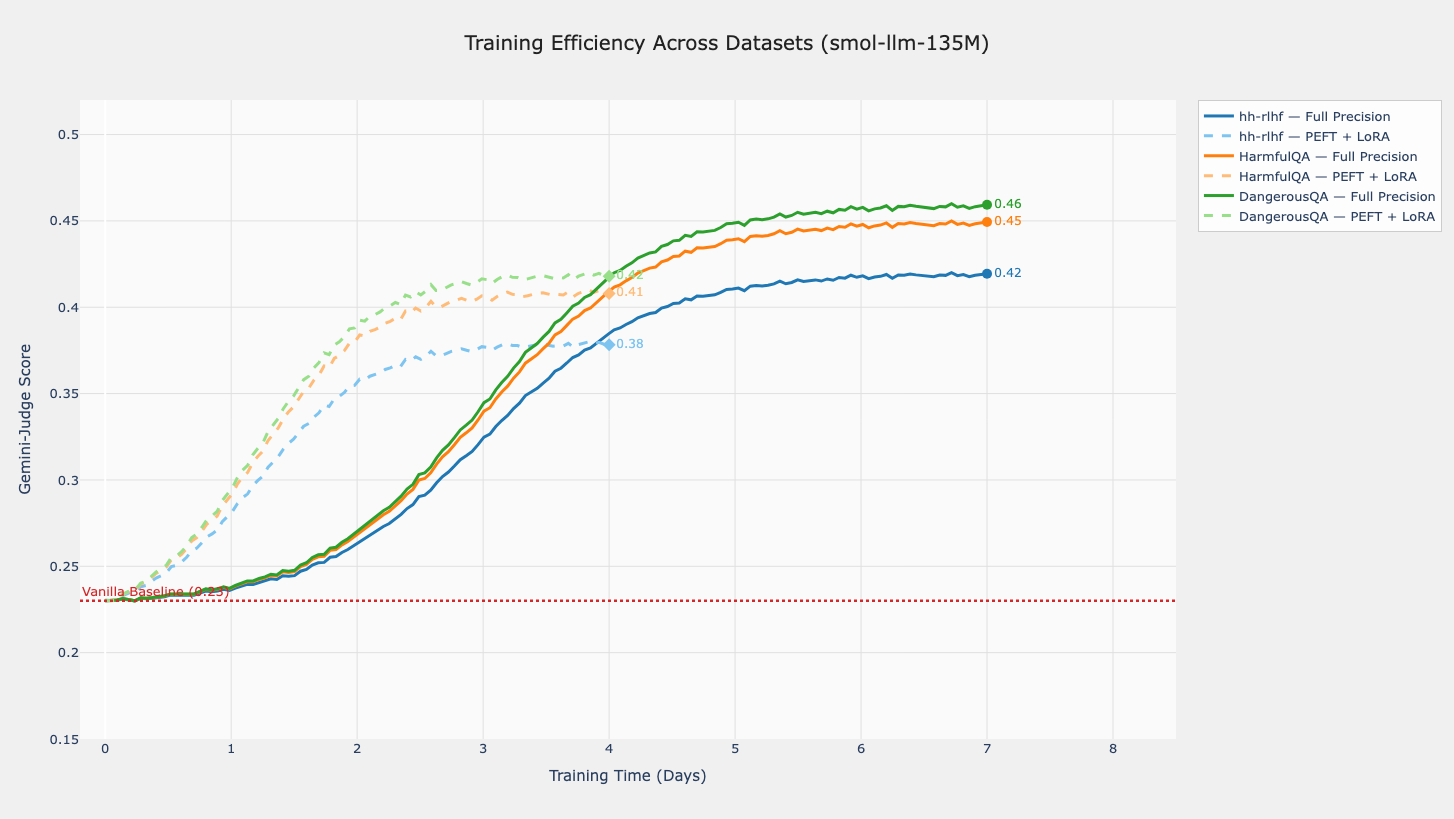
\includegraphics[width=\linewidth]{benchplot.png}
\caption{Training efficiency comparison for SmolLM-135M. PEFT+LoRA reaches lower but comparable Gemini-judge scores after roughly four days, while full precision continues to improve until roughly seven days.}
\label{fig:benchplot}
\end{figure}

The dashed PEFT+LoRA curves rise faster during the first two to three days, then level off around 0.38--0.42 depending on the dataset. The full-precision curves start slower but keep improving until the seven-day endpoint. LoRA cuts about three days from the run, roughly 43\% of the full-precision schedule. The likely explanation is that adapter tuning captures the easier safety corrections early, while full precision keeps finding smaller gains with longer optimization.

\begin{table}[H]
\centering
\caption{Estimated peak VRAM for full fine-tuning and LoRA fine-tuning on SmolLM-135M.}
\label{tab:vram-comparison}
\begin{tabular}{lc}
\toprule
Mode & Estimated peak VRAM \\
\midrule
Full fine-tuning & about 2.5--3.5 GB \\
LoRA fine-tuning & about 0.9--1.5 GB \\
\bottomrule
\end{tabular}
\end{table}

Table~\ref{tab:vram-comparison} gives the estimated peak VRAM. LoRA uses less memory because it updates only the adapter weights and their optimizer states, not the full model.

\subsection{Statistical analysis}
The available results are single-run, dataset-level scores rather than repeated-seed or prompt-level paired outcomes. We therefore treat them as descriptive. The pattern is still useful: LoRA trails full fine-tuning by 0.04 judge-score points on each dataset and finishes about three days earlier.

\section{Discussion}
\label{sec:discussion}

\subsection{Expected improvement}
The improvement from PEFT/LoRA is practical, not purely score-based. Full fine-tuning remains the stronger baseline because it can update the whole model. LoRA is useful if it gets close enough at a much lower cost. For this assignment, that tradeoff matters more than a small difference in judge score.

\subsection{Why LoRA may work}
IterAlign trains on revised answers to harmful prompts. That signal may not require broad changes to the whole model. Many safety behaviors are changes in instruction-following style, refusal wording, and response framing. LoRA is built for that kind of targeted adaptation: it changes behavior through low-rank updates while leaving the pretrained weights fixed.

\subsection{Why LoRA may fail}
LoRA can still underperform. Some harmfulness reductions may require deeper changes than rank-16 adapters can represent. The small base model may also lack the capability to produce safe and useful answers after only adapter tuning. Another risk is noisy oracle output. If the induced constitutions or revised answers are weak, the fine-tuning method cannot fix the data.

\subsection{Limitations}
The main limitations are:
\begin{itemize}
  \item The experiment uses a much smaller model than the original IterAlign paper.
  \item Gemini 3.1 Flash Lite is not the same oracle used in the original paper.
  \item Results may be descriptive rather than statistically significant if only one run is completed.
  \item DangerousQA tests a different harm distribution from the other reproduction datasets.
  \item PEFT improves efficiency, but it does not remove dependence on oracle judging.
\end{itemize}

\subsection{How final results should be interpreted}
The best possible outcome would have been for LoRA to match full fine-tuning exactly. It does not. The result is still useful: LoRA gives up 0.04 judge-score points on each dataset, cuts the schedule from about seven days to about four, and updates only adapter weights. For a course-scale reproduction, that is a reasonable trade.

DangerousQA is the additional-dataset test. LoRA has the same 0.04 gap there that it has on hh-rlhf and HarmfulQA, so the tradeoff does not appear to be limited to one prompt distribution.

\section{Conclusion}
\label{sec:conclusion}

Assignment 3 extends our IterAlign reproduction by targeting its most practical weakness: repeated full fine-tuning is expensive. The PEFT/LoRA version keeps the failure-driven constitution loop intact and replaces full-model updates with adapter tuning. In the current results, LoRA preserves most of the alignment gain, reduces training time, and updates only a small adapter parameter set. That makes IterAlign more realistic for small research environments.

\bibliographystyle{plain}
\bibliography{refs}

\end{document}
